\chapter{Future Work}
As mentioned in Conclusion Chapter, in the future, the whole workflow can be completed according to the current  techniques used in this project. It will enable YuMi to complete more holes up to finishing the entire shoe. In this chapter, several alternative methods to address the shoelace manipulation problem are discussed. 


\section{Gripper or External Wrist Camera} \label{futurecamera}

\begin{figure}[H]
\centering
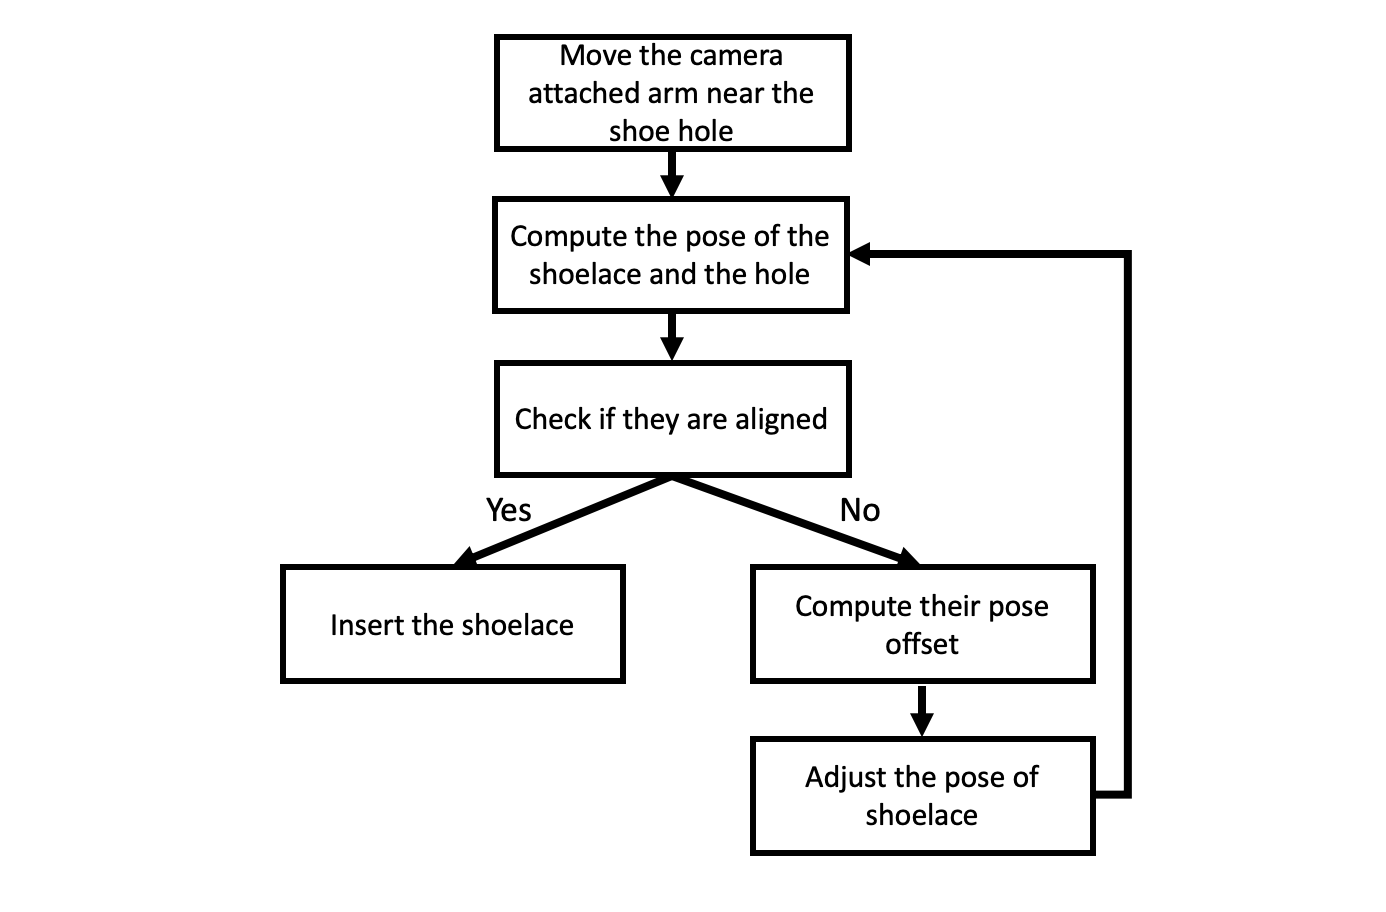
\includegraphics[width = 0.8\columnwidth]{Futurework/feedbackcamera.png}
\caption{}
\label{feedbackcamera}
\end{figure}
Due to the reason that gripper camera of YuMi is currently unavailable, and attaching another small camera on YuMi's arm will limit YuMi's motion, this project only used one workspace camera eventually. When the gripper cameras become available or a suitable attaching way for wrist camera is found, a more robust computer vision algorithm can be implemented, as shown in Figure \ref{feedbackcamera}.

For this approach, the wrist camera will detect and calculate the pose of shoe hole and shoelace, and only perform insertion if they are aligned. Ideally, this will improved the success rate of insertion task to 100\%. However, due to the additional computation and alignment, the execution time is considered to increase, which is the main drawback. 

\section{Shoe Model Construction}
As mentioned in Section \ref{oriestimation} of Background Chapter, there are numbers of existing methods to estimate the 6D pose of objects. By building shoe dataset that contains the photos and labels, and then retaining these models, the 6D pose of shoe can be computed in real-time. 

After that, the 3D model of manipulated shoe need be constructed, which should contain the relative pose between every shoe hole and the centroid of the shoe. By doing this, once the pose estimation model gives the 6D pose of the shoe, every hole's pose can be determined accordingly. The motion planning algorithm can be applied directly afterwards. This approach is a combination of shoe detection, 3D location estimation and 3D orientation estimation discussed in this report. Adv

\section{Deformable Object Tracking}


\section{Reinforcement Learning}